The architecture of the Wheel Share system is intended at developing scalable, secure, user-friendly ride sharing service that may be used by multiple users Rider, Driver, and Admin to serve in each of the mobile and web environments. The chapter gives a summary of the architectural structure, design limitations, and approach to be used in order to provide an unhindered user experience, performance of the system, and flexibility to experience future expansion. Since Wheel Share incorporates real-time data processing and cloud-based systems, it was stressed that proper planning and modular design were necessary to ensure that the system was efficient, had a high level of maintainability, and reliability of all the components\cite{mitropoulos2021}.


\section{System Architecture}
Wheel Share system is based on a service-oriented architecture that is modular to guarantee flexibility and scalability. It uses Flutter to develop cross-platform front-end forms, which could serve both mobile and web consumers. The client connects to Supabase services Authentication, PostgreSQL Database, and Storage, and Realtime channels via secure HTTP connections via JWT-modified sessions. 
The PostgreSQL uses Row-Level Security (RLS) policies to provide Role-Based Access Control (RBAC) to guarantee that users can only retrieve data that they are allowed to access by their role.  

A database has information that is important (user profiles, ride details, offers, emergency alerts, and so on) whereas Supabase storage has media files such as ride pictures or payment receipts. The use of this architecture provides secure communication, reliable data storage and real time synchronization of rides, offers and emergency notifications throughout the platform\cite{taiebat2022}.

\begin{figure}[H]
    \centering
    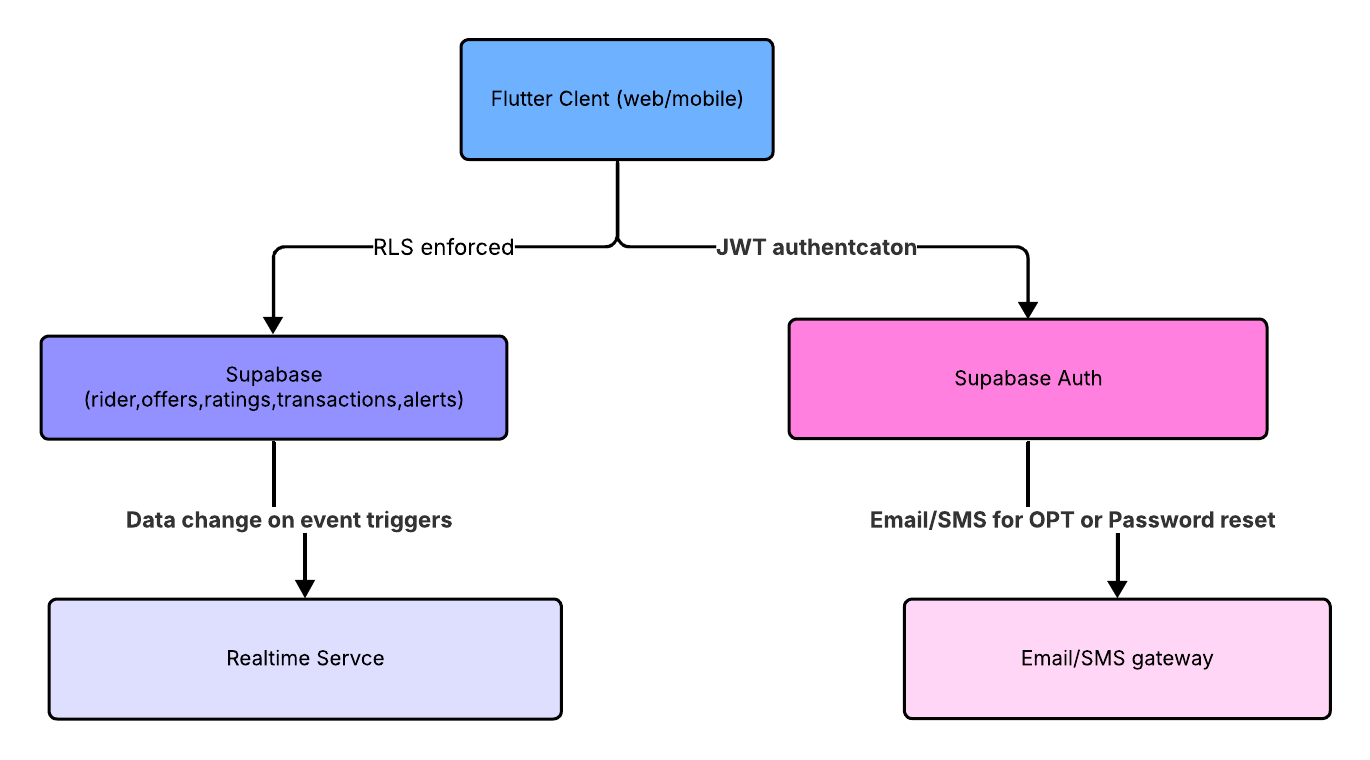
\includegraphics[width=0.9\textwidth,height=0.5\textheight]{Thought web weaver.png} 
    \caption{System Architecture Design}
    \label{fig:system-architechture-diagram}
\end{figure}
\noindent
\textbf{Description:} This architecture illustrates the interaction between the Flutter client, Supabase backend, and authentication services. The Flutter web/mobile client communicates with Supabase using JWT-based authentication, where Row Level Security (RLS) ensures controlled data access. Supabase Auth manages user authentication and handles email based OTP and password reset through an external gateway. Any data changes in the Supabase database trigger real-time services, enabling instant updates for rides, offers, ratings, transactions, and emergency alerts within the system.



\section{Design Constraints}
When designing Wheel Share, there were a number of technical, environmental, and operational factors that were used to design the system in a manner that satisfies its operation in the real-life state. 

\begin{itemize}
    \item \textbf{Software Requirements:} The browser Wheel Share should be compatible with latest software like Google Chrome or Microsoft Edge or Android mobile platforms. The communication with Supabase services through HTTPS requires a stable internet connection. Moreover, authentication and password recovery messages will also need an organization email account. 
    \item \textbf{Development Environment Requirements:} The programming languages needed in the front-end development are Flutter SDK (greater than 3.x) and Dart programming language. IDEs: the IDEs may be VS Code or Android Studio. It can be run with the aid of the backend using Supabase, and formatted with the help of SQL migration tools with the help of web-based Supabase Dashboard
    \item \textbf{Frameworks and Programming Language:} The front-end Flutter Dart of the system is reactive and has the successful state management. It also has a Supabase-based backend which contains PostgreSQL and structured data storage, Authentication and secure user management, storage and media management, and real-time updates. In addition, emergency alerts and receive notifications both will be the secure workflows that will be implemented on serverless Edge Functions. 
     \item \textbf{Technical Limitations:} Storage space and network latency of mobile browsers are also restricted by limitations of system performance, therefore, can have an impact on real-time ride updates and notifications. Besides, real time capabilities scalability depends on Supabase project which are the number of concurrent WebSocket connections and the number of concurrent requests.
     \item \textbf{Assumptions:} I believe the user familiar with the cardinal ride-sharing is involved in the activities of posting rides, making and accepting offers and rating rides. The fact that the drivers are supposed to be aware of the availability of the rides also questions them assuming that the emergency alerts will be monitored by the administrators at any given time. 

\end{itemize}

\section{Design Methodology}
The Wheel Share development and design process is modular and structure based which is premised on an \textbf{Agile development methodology}. The system is divided into logical modules that are easy to understand and they can be maintained at the same time as they can be developed.
\begin{itemize}
    \item \textbf{Partitioning: } The system is separated by features into Rider, Driver, and Admin modules and has some common services like Authentication, Ride Management, and Notifications. The database is partitioned to use separate tables that contain the data of the Users, Rides, Offers, Ratings, Transactions, and Emergency Alerts. Time based partitioning is used to manage asynchronous jobs such as the summary of earnings or expenditure and the delivery of timely notifications. 
    \item \textbf{Communication Requirements:} Communication between the client and Supabase is fully complete via the HTTPS protocol using tokens through in the authorization header. Instant synchronization, e.g. new offers, ride confirmations and emergency alerts are handled through WebSocket channels. 
    \item \textbf{Agglomeration Strategy:} Shared ride-list, offer management and rating display UI widgets are used to achieve design efficiency and re-usability of code. Database views are developed to make complex queries easier. 
    \item \textbf{Mapping:} Flutter has route guards that are mapped to role based permissions to ensure that only Riders, Drivers and admin can gain access of an authorized section. Database entities like Rides and Offers are implemented with RLS policies, and Edge Functions are implemented to automatically notify the administrator and emergency contacts in case an alert is fired. 

\end{itemize}

\begin{figure}[H]
    \centering
    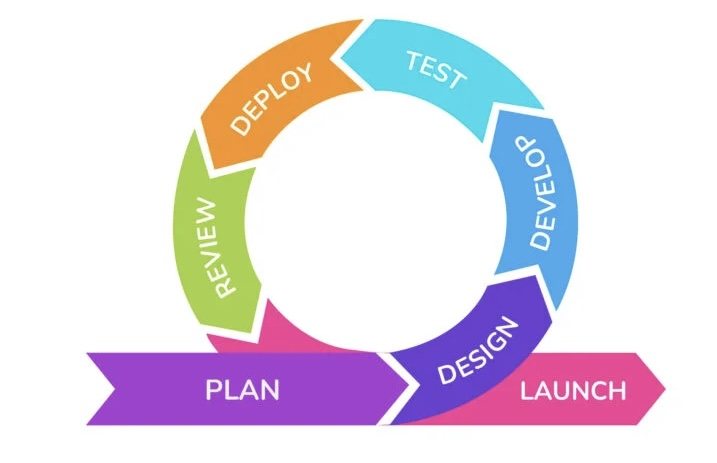
\includegraphics[width=0.6\textwidth]{agile.jpg} 
    \caption{Agile Methodology}
    \label{fig:agile-methodology-diagram}
\end{figure}

\section{High-Level Design}

The high level design of Wheel Share names the key elements of the system and their interaction process to attain the desired functionality. It focuses primarily on the database design and entity relationships, which guarantee efficient storage, retrieval and connectivity of the information of the user and the ride. 

\begin{itemize}
 \item \textbf{User:} Keeps information about customers like user-Id, name, email, role- Rider/Driver and profile description. 
 \item \textbf{Ride:} Ride data are stored in the stores and include ride related data such as source, destination, city, address, date and rider identification. 
 \item \textbf{Provide:} Relates rides/drivers and offers four fields of offer-Id, ride-Id, driver-Id and offer-Status.
 \item \textbf{Rating:} : It is used in rating the rides and is contained of rating-Id, ride-Id, reviewer-Id, score, and comments. 
 \item \textbf{Transaction:} : This table records all the transactions by transaction-Id, ride-Id, user-Id, amount and type (earning/ spending). 
 \item \textbf{Emergency Alert:} : Responsible of handling alerts like alert-Id,ride-Id,timestamp and status. 
\end{itemize}
\clearpage

\subsection{User Login Authentication and Authorization Flow}


\begin{figure}[H]
    \centering
    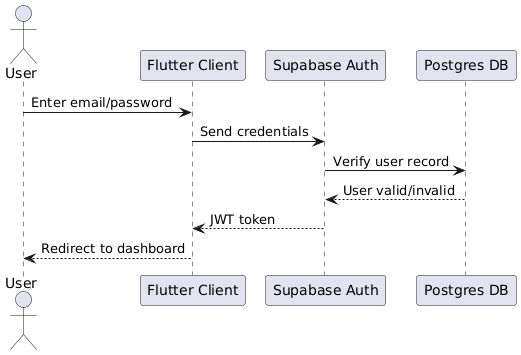
\includegraphics[width=1.0\textwidth]{HLD 1.png}
    \caption{User Login Sequence Diagram Using Flutter and Supabase Authentication}
    \label{fig:Sequence-diagram}
\end{figure}

\noindent
\textbf{Description:} This sequence diagram shows the user login process in the system. The user enters credentials through the Flutter client, which are sent to Supabase Authentication for verification. Supabase Auth validates the user using the PostgreSQL database. After successful authentication, a JWT token is generated and the user is redirected to the dashboard.
\clearpage


\subsection{Ride Posting and Real-Time Notification Flow}


\begin{figure}[H]
    \centering
    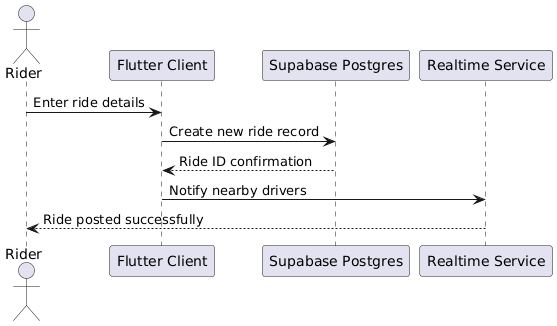
\includegraphics[width=1.0\textwidth]{HLD 2.png}
    \caption{Ride Posting Sequence Diagram}
    \label{fig:ride-posting-sequence}
\end{figure}

\noindent
\textbf{Description:} This sequence diagram illustrates the ride posting process performed by a rider. The rider enters ride details through the Flutter client, which creates a new ride record in the Supabase PostgreSQL database. Once the ride is successfully stored, a ride ID is generated. The real-time service then notifies nearby drivers about the newly posted ride.
\clearpage



\subsection{Offer Management and Ride Confirmation Flow}


\begin{figure}[H]
    \centering
    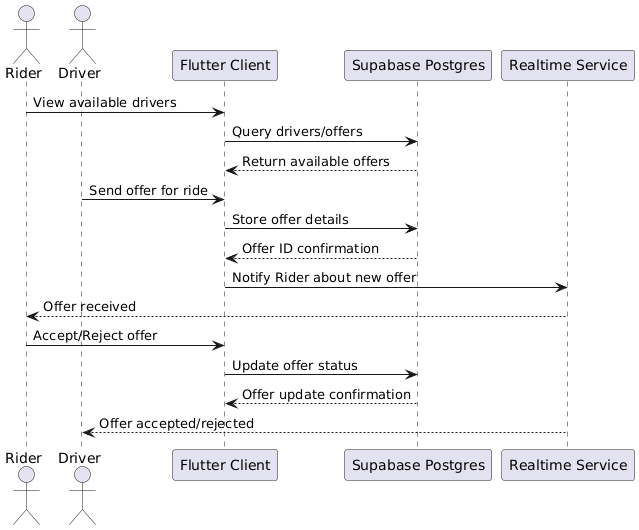
\includegraphics[width=1.0\textwidth]{HLD 3.png}
    \caption{Offer Management Sequence Diagram}
    \label{fig:offer-management-sequence}
\end{figure}

\noindent
\textbf{Description:} This sequence diagram shows the offer management process between riders and drivers. Drivers view available rides and send offers through the Flutter client, which are stored in the Supabase PostgreSQL database. The real-time service notifies riders about new offers. Riders can accept or reject offers, and the system updates the offer status accordingly.
\clearpage


\subsection{Emergency Alert Handling and Notification Flow}


\begin{figure}[H]
    \centering
    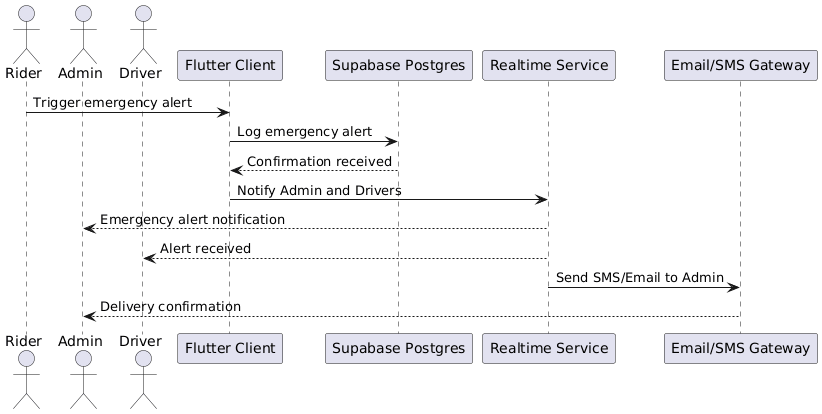
\includegraphics[width=1.0\textwidth]{HLD 4.png}
    \caption{Emergency Alert Handling Sequence Diagram}
    \label{fig:emergency-alert-sequence}
\end{figure}

\noindent
\textbf{Description:} This sequence diagram illustrates how emergency alerts are handled within the system. When a rider triggers an emergency alert, the Flutter client logs the alert in the Supabase PostgreSQL database. The real-time service notifies the admin and drivers instantly, while the Email/SMS gateway sends notifications to ensure timely response and user safety.



\section{Low-Level Design}

Each system component's specific structure is specified in the WheelShare Low-Level Design. With distinct interfaces and internal logic, it divides the program into smaller parts, including ride posting, ride search, offer handling, emergency alarms, admin monitoring, and authentication. In addition to offering a clear implementation plan, this modular approach guarantees that the code is simple to create, maintain, and reuse.
\clearpage
\subsection{Post Ride Submission and Validation Workflow}


\begin{figure}[H]
    \centering
    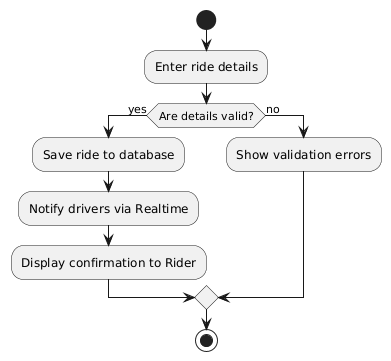
\includegraphics[width=1.0\textwidth]{LLD 1.png} 
    \caption{Post Ride Process Activity Diagram}
    \label{fig:post-ride-activity}
\end{figure}

\noindent
\textbf{Description:} This activity diagram represents the workflow of posting a ride in the system. The rider enters ride details, which are first validated by the system. If the details are valid, the ride is saved to the database and nearby drivers are notified through the real-time service; otherwise, validation errors are displayed to the rider.

\clearpage
\subsection{Ride Offer Acceptance and Rejection Workflow}


\begin{figure}[H]
    \centering
    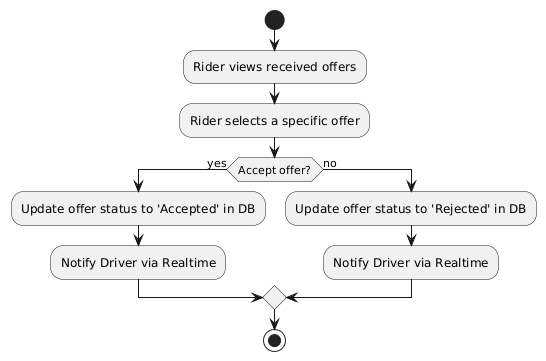
\includegraphics[width=1.0\textwidth]{LLD 2.png} 
    \caption{Accept Offer Process Activity Diagram}
    \label{fig:accept-offer-activity}
\end{figure}

\noindent
\textbf{Description:} This activity diagram illustrates the process of handling ride offers by the rider. The rider views received offers and selects a specific offer to accept or reject. Based on the decision, the system updates the offer status in the database and notifies the driver in real time.





\section{GUI Design}
Wheel Share is built with Flutter as its Graphical User Interface (GUI) to provide a similar and dynamic experience in the mobile and web interfaces. The interface is centered upon the clarity, access and ease of navigation. A bottom navigation bar or a layout based on tabs enables the users to have a quick reach to the basic functions such as posting rides, looking at offers, checking the earnings or spending, and causing emergency notifications. It is minimalistic and easy to use in design: there are no icons or labels, the color schemes are balance-oriented, and the input forms fit on a mobile screen. The system can also incorporate real-time notification of offers, confirmation and alerting to ensure continuous information to the users.  

\section{Mobile App Interface}

The Flutter-based GUI was developed with a focus on:


\subsection{Initial App Launch and Location Permission Screen}


\begin{figure}[H]
    \centering
    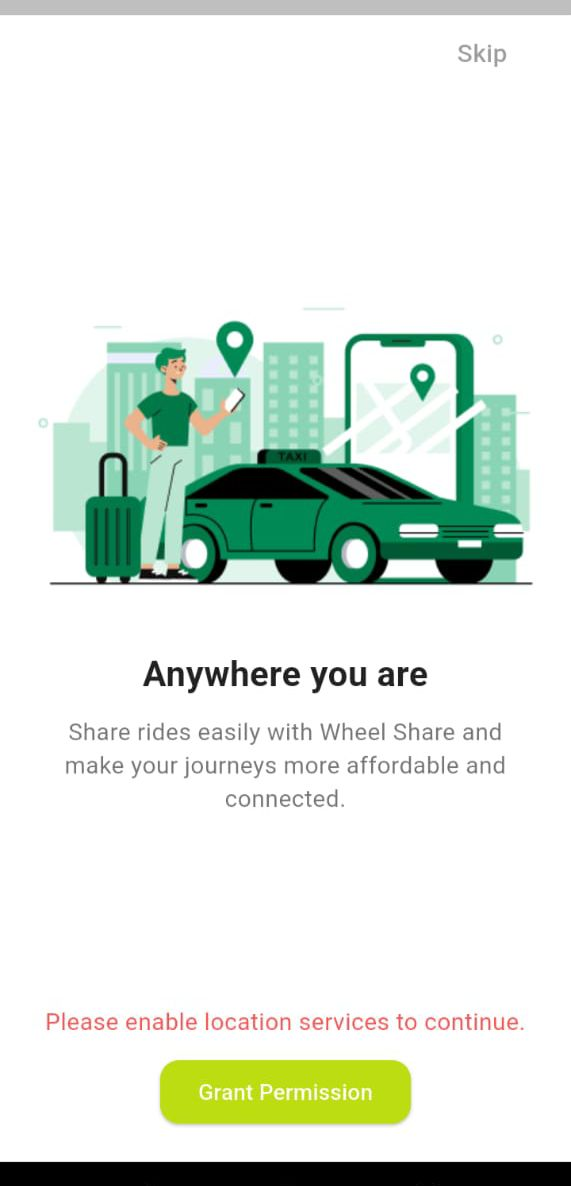
\includegraphics[width=0.6\textwidth,height=16cm]{frontt.jpeg} 
    \caption{Initial screen displayed when the application is installed}
    \label{fig:initial-app-screen}
\end{figure}

\noindent
\textbf{Description:} This screen is displayed when the application is launched for the first time after installation. It requests location permission to enable nearby ride discovery and navigation features.
\clearpage


\subsection{User Registration (Sign Up) Interface}


\begin{figure}[H]
    \centering
    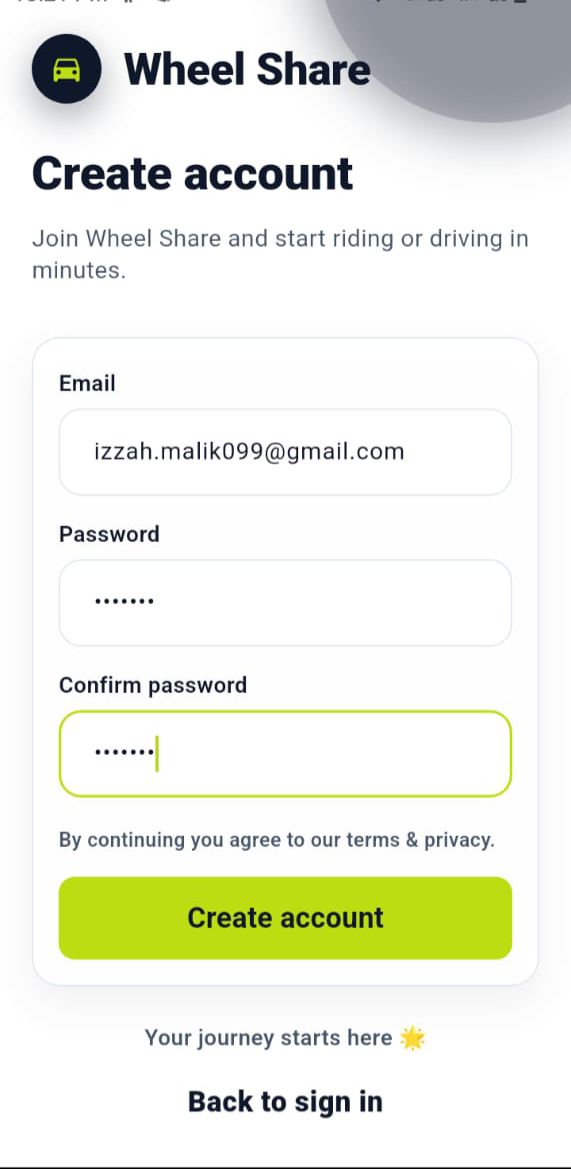
\includegraphics[width=0.6\textwidth,height=17.5cm]{sign.jpeg} 
    \caption{Sign Up Page}
    \label{fig:signup-gui}
\end{figure}

\noindent
\textbf{Description:} This interface enables new users to register by providing their email and password information. Upon successful registration, users gain access to the core functionalities of the application.
\clearpage


\subsection{ Admin Dashboard and System Monitoring Interface}


\begin{figure}[H]
    \centering
    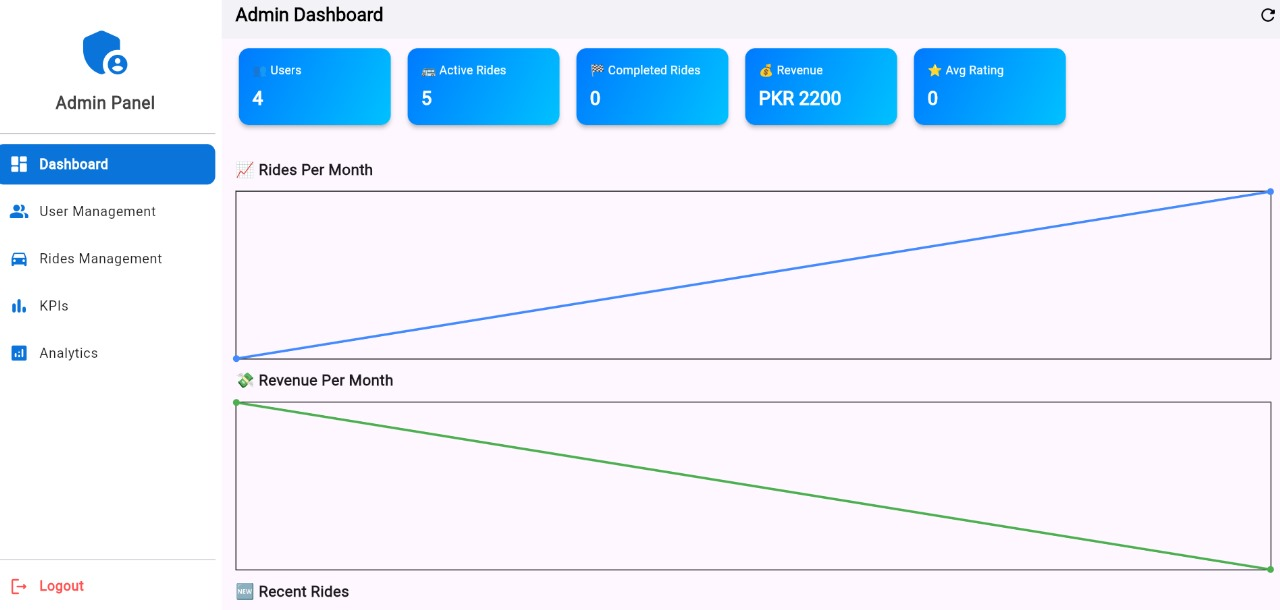
\includegraphics[width=0.9\textwidth,height=16cm]{WhatsApp Image 2025-11-24 at 6.47.08 PM.jpeg}
    \caption{Admin Page}
    \label{fig:admin-gui}
\end{figure}

\noindent
\textbf{Description:} This dashboard allows the admin to monitor system activity, including users, rides, and revenue statistics. It also provides analytical insights through graphs to support system management and decision-making.
\clearpage


\subsection{User Authentication (Login) Interface}


\begin{figure}[H]
    \centering
    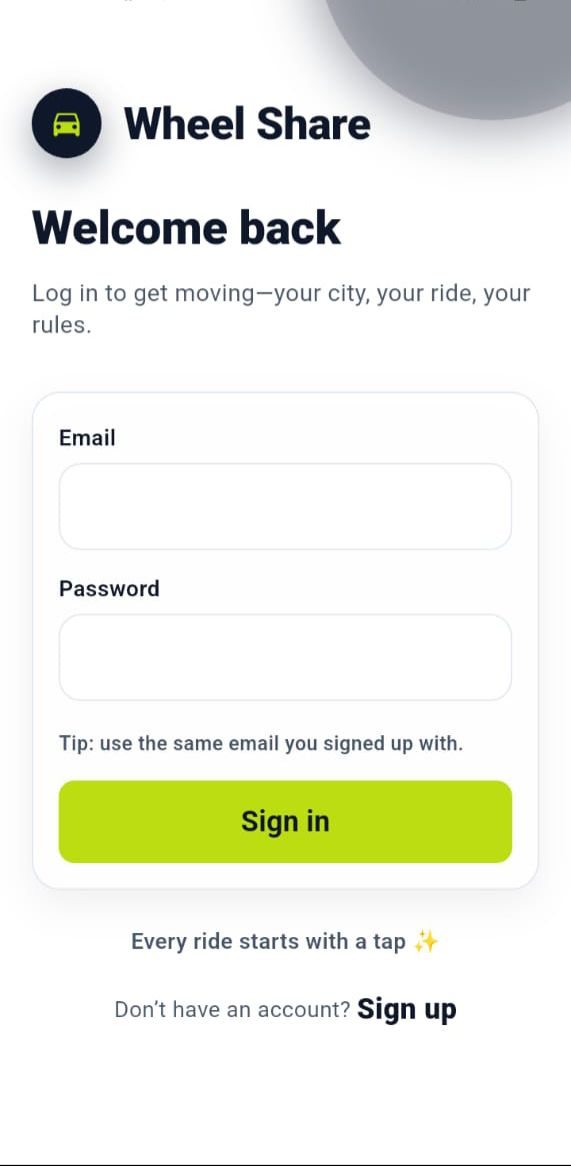
\includegraphics[width=0.6\textwidth,height=17.5cm]{loginp.jpeg} 
    \caption{Login Page}
    \label{fig:login-gui}
\end{figure}

\noindent
\textbf{Description:} This screen allows registered users to log in by entering their email and password credentials. Successful authentication grants access to personalized dashboards and ride-sharing features.
\clearpage



\subsection{User Profile and Account Information Interface}


\begin{figure}[H]
    \centering
    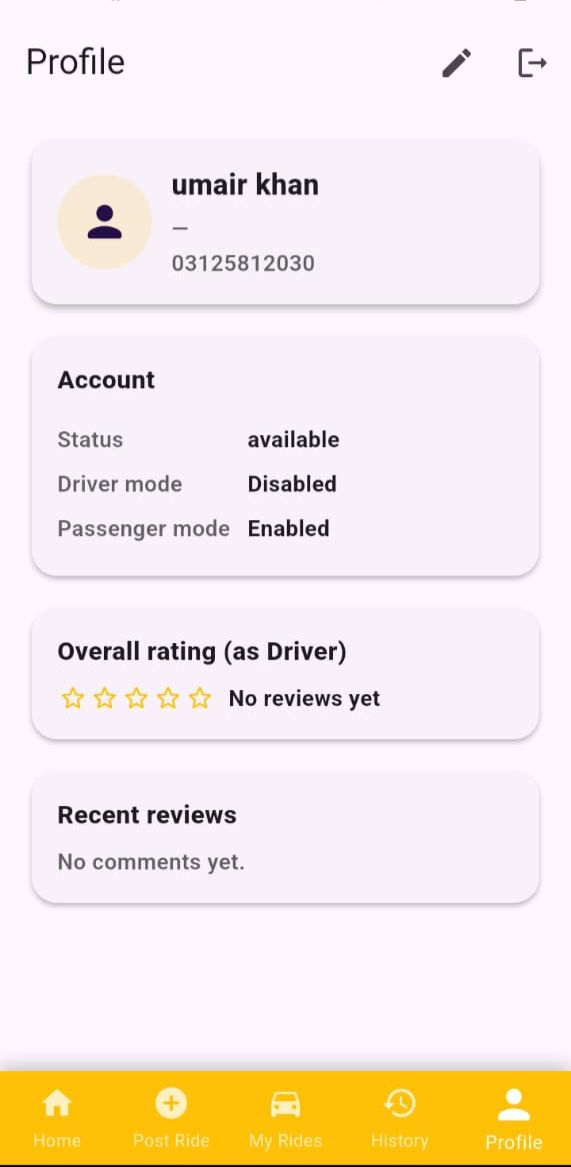
\includegraphics[width=0.6\textwidth,height=17.5cm]{user.jpeg} 
    \caption{User Profile}
    \label{fig:user-profile-gui}
\end{figure}

\noindent
\textbf{Description:} This screen displays the user’s personal details, account status, and role preferences. It also shows driver ratings and recent reviews to support trust and transparency within the system.
\clearpage


\subsection{Ride Posting Interface}


\begin{figure}[H]
    \centering
    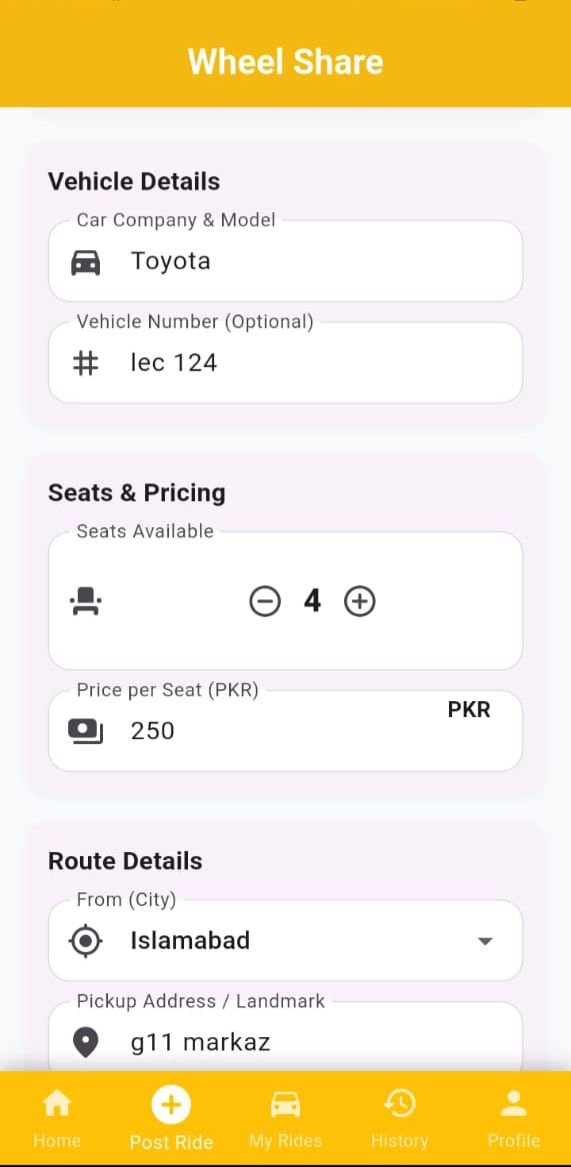
\includegraphics[width=0.6\textwidth,height=17.5cm]{ride posted.jpeg} 
    \caption{User Post Ride}
    \label{fig:post-ride-gui}
\end{figure}

\noindent
\textbf{Description:} This interface allows users to post a ride by entering vehicle, pricing, and route details. Once submitted, the ride becomes available for drivers or passengers to view and join.
\clearpage

\subsection{Location Selection for Ride Posting}


\begin{figure}[H]
    \centering
    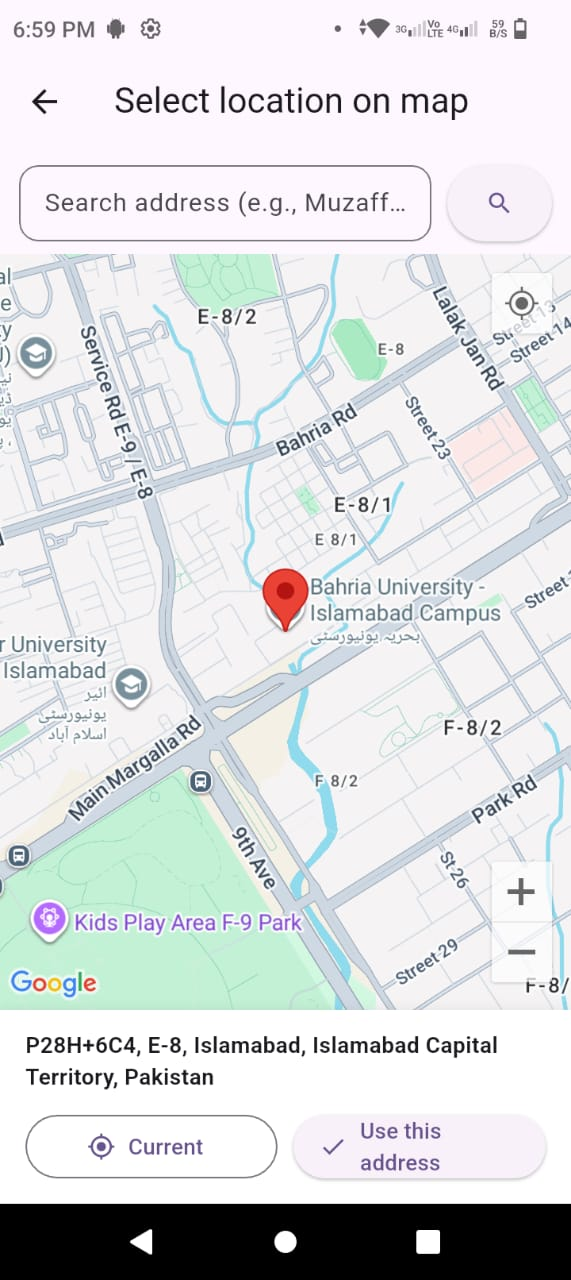
\includegraphics[width=0.6\textwidth,height=17.5cm]{WhatsApp Image 2025-12-14 at 7.00.35 PM.jpeg} 
    \caption{Map-Based Location Selection Screen}
    \label{fig:location-selection-gui}
\end{figure}

\noindent
\textbf{Description:} This screen allows users to select the pickup or destination location directly from the map. The selected address is used to ensure accurate routing and ride matching within the system.
\clearpage



\subsection{Ride Details and Availability Interface}


\begin{figure}[H]
    \centering
    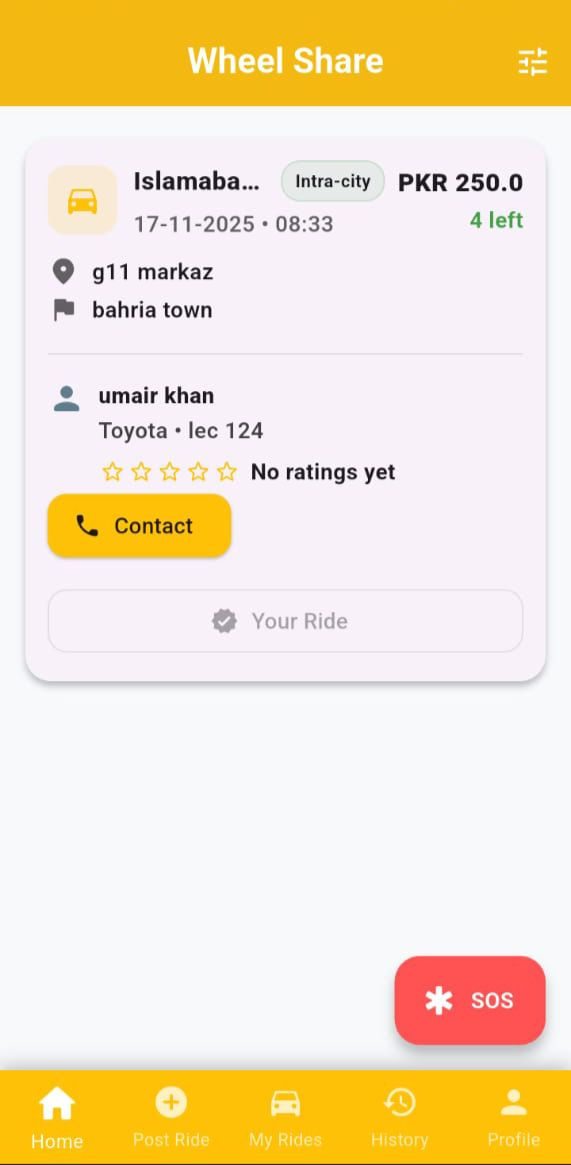
\includegraphics[width=0.6\textwidth,height=17.5cm]{avail.jpeg} 
    \caption{Ride Sharing Details}
    \label{fig:ride-details-gui}
\end{figure}

\noindent
\textbf{Description:} This screen displays detailed information about an available ride, including route, time, price, and driver details. Users can contact the driver or view ride status directly from this interface.
\clearpage


\subsection{Driver Ride Management Interface}


\begin{figure}[H]
    \centering
    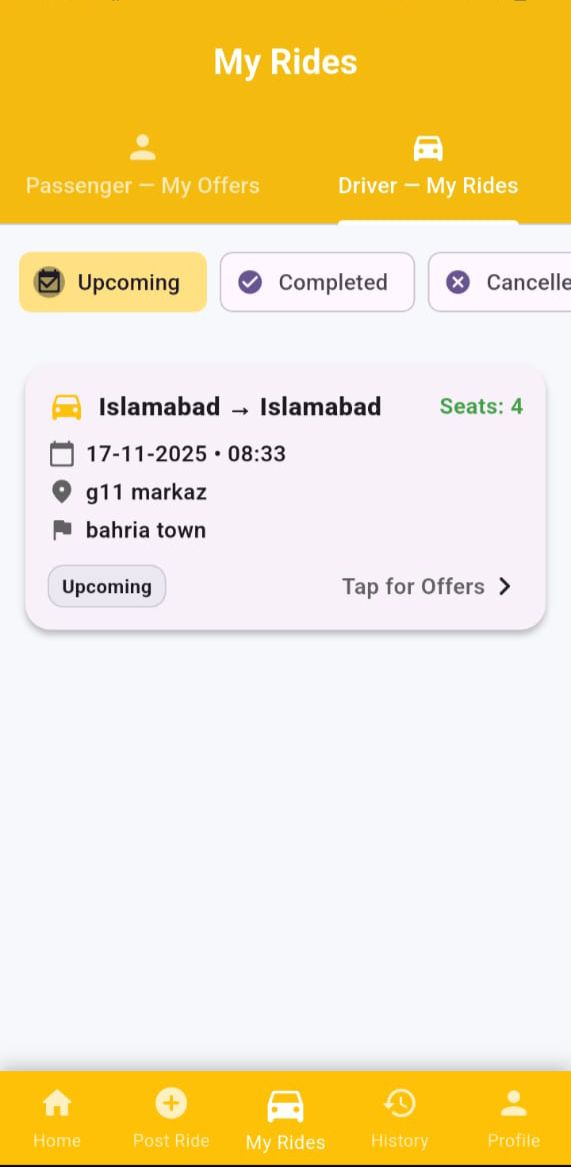
\includegraphics[width=0.6\textwidth,height=17.5cm]{dr ofer.jpeg} 
    \caption{Driver Offer a Ride}
    \label{fig:driver-offer-gui}
\end{figure}

\noindent
\textbf{Description:} This screen allows drivers to view and manage their posted rides, including upcoming and completed trips. Drivers can also review ride details and track available seats from this interface.
\clearpage


\subsection{Passenger Ride Offers Dashboard}


\begin{figure}[H]
    \centering
    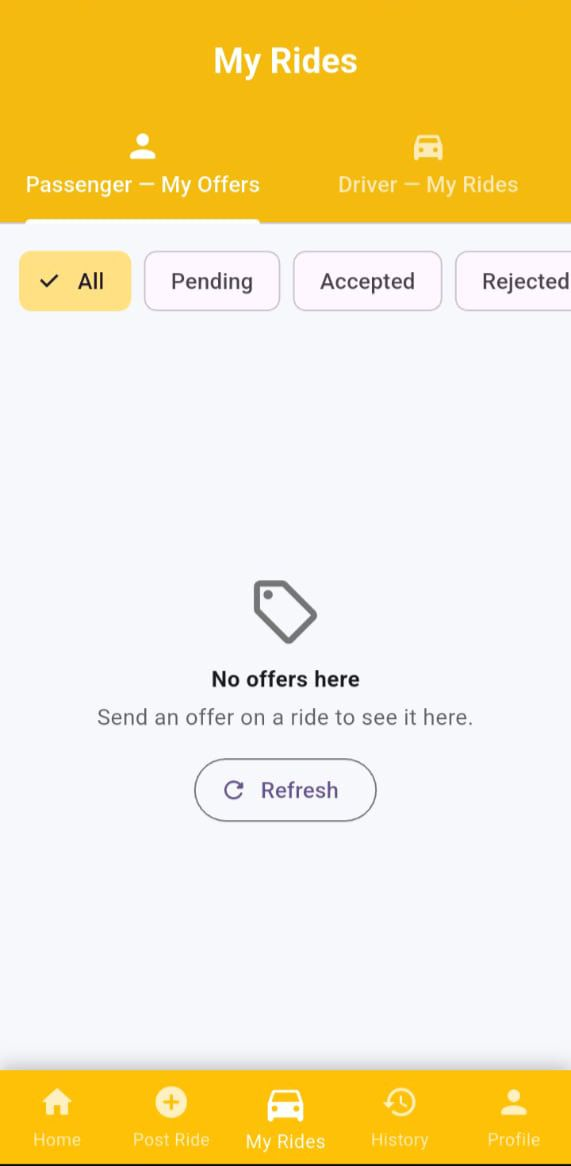
\includegraphics[width=0.6\textwidth,height=17.5cm]{psngr.jpeg} 
    \caption{Passenger Dashboard}
    \label{fig:passenger-dashboard-gui}
\end{figure}

\noindent
\textbf{Description:} This dashboard allows passengers to view and manage ride offers they have sent or received. Offers can be filtered by status such as pending, accepted, or rejected for easy tracking.
\clearpage

\subsection{History Dashboard}


\begin{figure}[H]
    \centering
    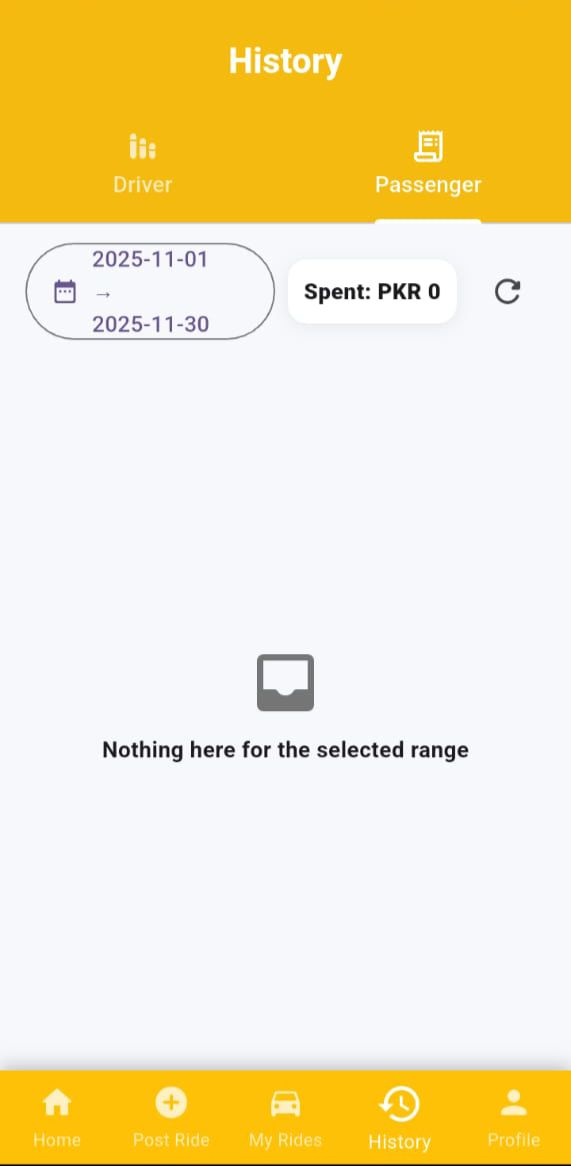
\includegraphics[width=0.6\textwidth,height=17.5cm]{his.jpeg}
    \caption{History Dashboard}
    \label{fig:history-dashboard-gui}
\end{figure}

\noindent
\textbf{Description:} This dashboard enables users to view their ride history within a selected date range and track total spending. If no rides exist for the chosen period, the system clearly indicates the absence of records.


\clearpage

\section{External Interfaces }
To provide a very efficient, safe and smooth experience Wheel Share works with various external services. Supabase is an authentication that provides user authentication, transactions, and passwords. Supabase database is a postgreSQL that handles operations related to ride, offers, transactions, and log emergency in addition to providing RLS as protection. 
The ride-related images, documents or receipts are stored securely by Supabase storage on signed URLs that provide limited access. The Realtime Service allows the use of the WebSocket channel on two-way communication to immediately update status, and the Email Gateways serve to notify about the offer acceptance, ride confirmations, and emergency messages. All external communication is carried out through the HTTPS or web socket protocols and the authentication is used to have secure and role-based access to data and integrity. 

 


